\section{Introduction}
One difficulty of the EAPM is 
to determine the target distributions.
This is called the problem of the convergence schedule or also called
the annealing schedule.
In related works,
one promising method is standard deviation schedule (SDS) 
\cite{thilo:sds,thilo:sds2}.
However, SDS is based on an empirical rule.

This chapter proposes a novel convergence schedule method and
highlights the theoretical aspects,
that is,
a relationship between the entropy of the target distribution
and the Fisher information, which can assess the
accuracy of the statistical estimation.
The proposed method is designed to improves the accuracy of the
statistical estimation.
The aim of this chapter is to investigate the 
efficiency of the proposed convergence schedule.



\section{Entropy Reduction Schedule (ERS)}
\subsection{Search Space Reduction}
The target distributions have an effect for
the variance of the importance sampling of (\ref{eapm-ml}).
The objective of the convergence schedule is to reduce the variance
of the importance sampling 
by controling the target distributions.

For simplicity, let us introduce two assumptions.
One is that
each probability model $p_t(x)$ completely approximates the corresponding 
target distribution $q_t(x)$, that is, $p_t(x)=q_t(x)$.
The other is that 
each target distribution is a partially uniform distribution.
For partially uniform distributions, 
the search space can be defined by $\Omega=\{x|q(x) \neq 0\}$.
It holds that $q(x)=\frac{1}{|\Omega|}$
for $x \in \Omega$
and $\Omega=Z$, where $Z$ is the normalizing constant.
Normally $\Omega_{t+1} \subseteq \Omega_t$ is satisfied in the EAPM,
 and then $x \in \Omega_{t+1}$ satisfies the following:
\begin{eqnarray}
 \frac{q_{t+1}(x)}{p_t(x)} 
=
 \frac{q_{t+1}(x)}{q_t(x)} 
= 
  \frac{|\Omega_{t}|}{|\Omega_{t+1}|}.
\label{ent_schedule_assume}
\end{eqnarray}
$(\frac{|\Omega_{t}|}{|\Omega_{t+1}|})^{-1}=
\frac{|\Omega_{t+1}|}{|\Omega_{t}|}$ can be
understood as the accept probability, which means
the probability of a sample generated from $\Omega_t$
to enter the region $\Omega_{t+1}$.
In importance sampling,
rejected samples that is $\frac{q_{t+1}(x)}{q_t(x)}=0$ (i.e., $x \not \in \Omega_{t+1}$)
have no effect,
and therefore a probability distribution
that maximizes the accept probability should be selected. 

In the EAPM,
multiple importance sampling are carried out.
The number of the accepted samples 
in a whole optimization process 
is written by
\begin{equation}
 \sum_{t=1}^{T} M_t \frac{|\Omega_{t+1}|}{|\Omega_{t}|},
\label{eq_sum_of_ap}
\end{equation}
where $M_t$ is the number of generated samples in the $t$-th iteration
and
$T$ is the number of the iterations.
By maximizing (\ref{eq_sum_of_ap}),
the following equations are obtained:
\begin{equation}
 M_{t-1}\frac{|\Omega_{t}|}{|\Omega_{t-1}|}=
 M_{t}\frac{|\Omega_{t+1}|}{|\Omega_{t}|}.
\label{eq_ers_max_cond}
\end{equation}
In general, $M_{t-1}=M_t$ and the equations are
rewritten by
\begin{equation}
\frac{|\Omega_{t+1}|}{|\Omega_{t}|}=c,
\label{eq_sp_reduction}
\end{equation}
where $0 \leq c \leq 1$ is a constant value, called the cutoff ratio.
(\ref{eq_sp_reduction}) is understood that
the size of search space is reduced with a common ratio $c$.


\subsection{Theoretical Justification}
The property of (\ref{eq_sp_reduction}) is intuitively good,
but there remains a question why (\ref{eq_sp_reduction})
is good from theoretical viewpoints.
For answering this question, 
the asymptotic error of MCI is highlighted.

In the EAPM, an expected log-likelihood, 
\begin{equation}
 L(\theta)=\int q(x) \log p(x|\theta),
\end{equation}
where $\theta$ is the parameter of the probability model $p(x|\theta)$,
is calculated via importance sampling as follows:
\begin{equation}
 \hat L(\theta) = \frac{1}{M} \sum_{p(x)} \frac{q(x)}{p(x)} \log p(x|\theta).
\end{equation}

The true parameter $\theta^*$, which maximizes $L(\theta)$, is satisfies
\begin{equation}
 \frac{\partial L}{\partial \theta}=E
\left[\frac{\partial}{\partial \theta}
  \log p(x|\theta^*)\right]_{q(x)}
=0.
\end{equation}
On the other hand, the variance 
\begin{eqnarray}
\sigma^2 &=& \mathrm{Var}
\left[\frac{\partial}{\partial \theta}
  \log p(x|\theta^*)\right]_{q(x)}\\
&=&
\mathrm{E}
\left[
\left(
\frac{\partial}{\partial \theta}
  \log p(x|\theta^*)
\right)^2
\right]_{q(x)}
\end{eqnarray}
is called the Fisher information and
becomes an assessment of the ML estimator.
In importance sampling, the Fisher information is calculated as follows:
\begin{eqnarray}
\sigma^2_{IS} &=& \mathrm{Var}
\left[\frac{q(x)}{p(x)}\frac{\partial}{\partial \theta}
  \log p(x|\theta^*)\right]_{p(x)}\\
&=&
\mathrm{E}
\left[
\left(
\frac{q(x)}{p(x)}
\frac{\partial}{\partial \theta}
  \log p(x|\theta^*)
\right)^2
\right]_{p(x)}.
\end{eqnarray}

By using the assumption of (\ref{ent_schedule_assume}),
the Fisher information in the EAPM is given by
\begin{eqnarray}
 \sigma^2_{IS}&=&\frac{\Omega_t}{\Omega_{t+1}}\sigma^2_t,
\end{eqnarray}
where $\sigma^2_t = \mathrm{Var}
\left[\frac{\partial}{\partial \theta}
  \log p(x|\theta^*)\right]_{q_t(x)}$.
This shows that the original Fisher information is multiplied by 
the inverse of the accept probability. 

The squared error,
\begin{equation}
\left|\frac{\partial \hat L(\theta^*)}{\partial \theta}
-\frac{\partial L(\theta^*)}{\partial \theta}\right|^2
=
\left|
\frac{\partial \hat L(\theta^*)}{\partial \theta}
\right|^2
\end{equation}
represents the empirical Fisher information.
According to (\ref{eq_mci_error}),
the average squared error is written with the accept probability as follows:
\begin{equation}
E\left[
\left|
\frac{\partial \hat L(\theta^*)}{\partial \theta}
\right|^2
\right]
=
\frac{\sigma_t^2}
{
\frac{\Omega_{t+1}}{\Omega_{t}}M_t
}.
\end{equation}
Here, it becomes clear that our maximization condition  
(\ref{eq_ers_max_cond}) minimizes the sum of the inverse\footnote{
The inverse of Fisher information has important aspect.
\begin{equation}
 \mathrm{Var}[\hat \theta] \geq \frac{1}{\sigma^2}
\end{equation}
is well known bound on any unbiased estimator
as Cram\'{e}r-Rao bound. 
}
 of Fisher
information, that is, 
\begin{equation}
\sum_t
{
\frac{\Omega_{t+1}}{\Omega_{t}}M_t
}
\frac{1}{\sigma_t^2},
\end{equation}
 however, 
under the assumption that each $\sigma^2_t$ for the $t$-th 
target distribution is equivalent to each other.  


\subsection{Search Space Size and Entropy}
In the previous section, 
we consider only the partially uniform distribution, 
and the concept of the search space $\Omega$ plays the central role. 
In the EAPM, we control other types of probability distributions 
such as Boltzmann distributions, and however
it seems to be difficult to define the search space for the Boltzmann
distribution.

Actually, the size of the search space can be approximately measured by 
entropy, which is defined as follows:
\begin{equation}
 S=-\int q(x) \log q(x) dx.
\end{equation}
This integration can be understood as the geometric average.
The geometric average of $q(x)$ with respect to $q(x)$ 
is given by
\begin{equation}
 \bar q = \exp \int q(x) \log q(x) dx.
\end{equation}
This is understood as
an approximation of a general probability distribution
by a partially uniform distribution.
Then, the search space size is given by
\begin{equation}
 |\Omega|= \log S.
\end{equation} 

Finally, from (\ref{eq_sp_reduction}),
the convergence schedule is given by
\begin{equation}
 S_{t+1} - S_t= \log c.
\end{equation}
Note that $0 \leq c \leq 1$ and $-\infty \leq \log c \leq 0$.
This shows that the entropy is linearly reduced.
Hence, the proposed schedule is called
the entropy reduction schedule (ERS).


\subsection{Implementation Issues}
In practice, the entropy cannot be calculated exactly,
except for uniform distributions.
In ERS, entropy is estimated by using MCI.
The following sections show the methods
to find a parameter value such that
the probability distribution has the given entropy
for the partially uniform distribution and the Boltzmann distribution.


\subsubsection{Partially Uniform Distribution}
\label{sec-ftilde}
For partially uniform distributions,
the entropy is given by
\begin{equation}
 S=\log Z.
\end{equation}
Then, the objective is to solve the following equation:
\begin{eqnarray}
 Z^*&=&\hat Z(\tilde f),\\
    &=&\frac{1}{M} \sum_{p(x)} \frac{\tilde q(x|\tilde f)}{p(x)}
\end{eqnarray}
where $Z^*$ is the given search space size,
$\hat Z$ is the estimated normalizing constant, and
$\tilde q(x|\tilde f)$ is defined by (\ref{truncation}).

The estimator of the normalizing constant is
a monotonically decreasing step function with respect to $\tilde f$,
and its change-points are given by $f(x_1) \cdots f(x_M)$, 
where $x_1 \cdots x_M$ are the given samples.
Thus, the solution is selected from $f(x_1) \cdots f(x_M)$.
Assuming \mbox{$f(x_1) < \cdots <f(x_M)$} without loss of generality,
we have the following:
\begin{equation}
\hat Z(\tilde f(x_{i+1}))=\hat Z(\tilde f(x_{i}))+\frac{1}{M \times p_m(x_{i+1})}.
\end{equation}
A linear search on $f(x_1) \cdots f(x_M)$
can afford an approximate solution.
In the experiments,
for $\tilde f$, we select $f(x_k)$
such that $\hat Z(f(x_k))-Z^*$ is minimized
under $Z^*<\hat Z(f(x_k))$.


\subsubsection{Boltzmann Distribution}
For Boltzmann distributions,
the entropy is given by
\begin{equation}
 S= \bar f \beta + \log Z,
\end{equation}
where $\bar f=\int q(x) f(x) dx$.
Its derivative is given by
\begin{equation}
 \frac{\partial S}{\partial \beta}= - \sigma^2 \beta,
\end{equation}
where $\sigma^2=\mathrm{Var}[f(x)]_{q(x)}$ and this can be
calculated via importance sampling.
Our approach is based on the gradient.
By using the assumption that $\sigma^2$ is a constant value,
the difference of the entropy is approximately given by
\begin{eqnarray}
 \Delta S &\simeq& - \sigma ^2 \int \beta \, d\beta.
\end{eqnarray}
Then, we obtain the update rule
\begin{equation}
 \beta_{t+1}=\sqrt{\beta_t^2 - \frac{\Delta S}{\sigma_t^2}}.
\end{equation}
This is the single step updating.
Of course we can employ a multi-step updating way.


\section{Experiments}
For the basic framework,
the resampling population model (RPM) \cite{higo:rpm} is employed
because it is experimentally confirmed that RPM is more efficient than
the EAPM.
the EAPM has one parameter that is
the number of generated samples in one sampling, denoted by $M$.
RPM has one additional parameter to the EAPM.
That is the number of the stored samples, denoted by $N$.
ERS has the parameter of the cutoff ratio defined in
(\ref{eq_sp_reduction}), and denoted by $c$.
The difference of entropy is obtained by $\Delta S = \log c$.




\subsection{Basic Property}
This section describes experiments conducted to investigate
 the basic property of ERS.
The parameters are setup as 
$N=200$, $M=200$, $c=0.1$ ($\Delta S= \log 0.1 \simeq 0.105$).
The parameters are experimentally determined so that
the Monte Carlo error is sufficiently ignored.
Two cases which employ the partially uniform distribution and 
the Boltzmann distribution, respectively, are experimented.


\subsubsection{Result}
The Left-hand side figures of 
Figs. \ref{figers-t_ers_0d}, $\cdots $, \ref{figers-ers_2d} show
the evolution of the entropy. 
In each figure, the vertical axis represents
the empirical entropy.
The horizontal axis represents 
the number of iterations.
In theory, the entropy is linearly reduced.
The difference is $\log 0.1 \simeq 0.105$ and
the line in each figure represents $y=0.105 x + b$, where
$b$ is fitted to the data.

For onemax, 
the theoretical entropy transition is almost realized in both cases,
that is, the partially uniform distribution and the Boltzmann
distribution cases.
However, for 1D and 2D Ising model,
the realized entropy transition is different from the theoretical one
in both cases.


We show the evolution of the standard deviation of the cost function
value of the generated samples in the right-hand side figure of each figure.
ERS with the partially uniform distribution,
the difficulty of adjusting the threshold parameter described in 
Section \ref{sec-ftilde}
depends on 
the variance of the cost function value of the generated samples.
ERS with the Boltzmann distribution assumes that 
the variance of the cost function value with respect to the current
target distribution is not changed if the $\beta$ is slightly moved.
The rapid change can be seen for 1D and 2D Ising model
and, at that time, the entropy is quickly decreased in both cases.

\begin{table}
\centering
%\small
\caption{Results of ER for Onemax.}
\begin{tabular}{|r|r|rr|rr|}
\hline
\multicolumn{1}{|c|}{N} & \multicolumn{1}{|c|}{c} & 
\multicolumn{2}{c|}{Best} & \multicolumn{2}{c|}{Evaluations} \\ \hline
100 & 0.1 & --397.4 &  (1.5) & 3409 &  (83.72) \\ \hline
500 & 0.1 & --400 &  (0) & 15500 &  (196.21) \\ \hline
1000 & 0.1 & --400 &  (0) & 30300 &  (788.67) \\ \hline
3000 & 0.1 & --400 &  (0) & 90300 &  (1728.58) \\ \hline
100 & 0.3 & --397.4 &  (0.92) & 3103 &  (86.38) \\ \hline
500 & 0.3 & --400 &  (0) & 14045 &  (260.24) \\ \hline
1000 & 0.3 & --400 &  (0) & 28030 &  (283.02) \\ \hline
3000 & 0.3 & --400 &  (0) & 82200 &  (1505.99) \\ \hline
100 & 0.5 & --397.1 &  (0.83) & 2750 &  (100) \\ \hline
500 & 0.5 & --400 &  (0) & 12650 &  (165.83) \\ \hline
1000 & 0.5 & --400 &  (0) & 24750 &  (460.98) \\ \hline
3000 & 0.5 & --400 &  (0) & 74100 &  (994.99) \\ \hline
100 & 0.7 & --394.5 &  (2.2) & 2397.7 &  (75.9) \\ \hline
500 & 0.7 & --400 &  (0) & 11004.9 &  (104.7) \\ \hline
1000 & 0.7 & --400 &  (0) & 21410.8 &  (523.08) \\ \hline
3000 & 0.7 & --400 &  (0) & 62401.7 &  (1639.37) \\ \hline
\end{tabular}
\label{result_0d_idea}
\end{table}

\begin{table}
\centering
\caption{Results of RTR ($C=0.7$) for Onemax.}
\begin{tabular}{|r|r|rr|rr|}
\hline
\multicolumn{1}{|c|}{N} & \multicolumn{1}{|c|}{M} & 
\multicolumn{2}{c|}{Best} & \multicolumn{2}{c|}{Evaluations} \\ \hline
10 & 10 & --255.9 &  (7.44) & 193 &  (16.16) \\ \hline
50 & 10 & --331.7 &  (5.9) & 2900010 &  (0) \\ \hline
50 & 50 & --370.9 &  (4.91) & 2900050 &  (0) \\ \hline
100 & 10 & --372.6 &  (4.78) & 2900010 &  (0) \\ \hline
100 & 50 & --390.1 &  (2.12) & 2900050 &  (0) \\ \hline
100 & 100 & --397.1 &  (1.81) & 2610730 &  (868110) \\ \hline
200 & 10 & --398.1 &  (1.22) & 2610823 &  (867561) \\ \hline
200 & 50 & --399 &  (0.89) & 2032990 &  (1324456.48) \\ \hline
200 & 100 & --399.7 &  (0.46) & 878810 &  (1323251.13) \\ \hline
200 & 200 & --400 &  (0) & 10820 &  (3552.41) \\ \hline
300 & 10 & --400 &  (0) & 18704 &  (3981.81) \\ \hline
300 & 50 & --399.9 &  (0.3) & 308135 &  (863982.34) \\ \hline
300 & 100 & --400 &  (0) & 18650 &  (2154.65) \\ \hline
300 & 200 & --400 &  (0) & 17320 &  (1695.76) \\ \hline
300 & 300 & --400 &  (0) & 18600 &  (2212.69) \\ \hline
\end{tabular}
\label{result_0d_rtr}
\end{table}

\vspace{0.5cm}

\begin{table}[tb]
\centering
\caption{Results of RPM ($C=0.01$) for Onemax.}
%\small
\begin{tabular}{|r|r|rr|rr|}
\hline
\multicolumn{1}{|c|}{N} & \multicolumn{1}{|c|}{M} & 
\multicolumn{2}{c|}{Best} & \multicolumn{2}{c|}{Evaluations} \\ \hline
10 & 10 & --267.8 &  (8.82) & 1455 &  (197.7) \\ \hline
50 & 10 & --395.7 &  (1.73) & 17935 &  (1268.47) \\ \hline
50 & 50 & --399.9 &  (0.3) & 118075 &  (4346.22) \\ \hline
100 & 10 & --400 &  (0) & 20291 &  (341.86) \\ \hline
100 & 50 & --400 &  (0) & 133730 &  (4321.41) \\ \hline
100 & 100 & --400 &  (0) & 313720 &  (9888.26) \\ \hline
200 & 10 & --400 &  (0) & 30225 &  (437.16) \\ \hline
200 & 50 & --400 &  (0) & 210360 &  (4185.08) \\ \hline
200 & 100 & --400 &  (0) & 476680 &  (8545.62) \\ \hline
200 & 200 & --398.8 &  (3.28) & 1040020 &  (122154.02) \\ \hline
300 & 10 & --400 &  (0) & 29187 &  (343.77) \\ \hline
300 & 50 & --400 &  (0) & 281865 &  (3792.63) \\ \hline
300 & 100 & --400 &  (0) & 609900 &  (11553.87) \\ \hline
300 & 200 & --400 &  (0) & 1319380 &  (23383.96) \\ \hline
300 & 300 & --397.3 &  (6.87) & 2019090 &  (315916.21) \\ \hline
\end{tabular}
\label{result_0d_rpm}
\end{table}

\begin{table}[tb]
%\small
\centering
\caption{The 5 best cases of RTR for 1D and 2D Ising. In all cases, the
 population does not converge and thus $2.9\times 10^6$ function
 evaluations are performed.}

(a) 1D Ising\\
\begin{tabular}{|r|r|r|rr|}
\hline
\multicolumn{1}{|c|}{N} & \multicolumn{1}{|c|}{M} & 
\multicolumn{1}{c|}{c} & \multicolumn{2}{c|}{Best} \\ \hline
200 & 200 & 0.3 & --370.2 & (5.55) \\ \hline
500 & 10 & 0.7 & --369.8 & (2.89) \\ \hline
200 & 10 & 0.3 & --369.6 & (3.07) \\ \hline
300 & 10 & 0.5 & --369.4 & (3.35) \\ \hline
500 & 500 & 0.7 & --369 & (3.13) \\ \hline
\end{tabular}

%\label{}
%\end{table}

\vspace{0.5cm}

%\begin{table}[tb]
(b) 2D Ising\\
\begin{tabular}{|r|r|r|rr|}
\hline
\multicolumn{1}{|c|}{N} & \multicolumn{1}{|c|}{M} & 
\multicolumn{1}{c|}{c} & \multicolumn{2}{c|}{Best} \\ \hline
500 & 300 & 0.7 & --733.4 & (9.96) \\ \hline
200 & 10 & 0.3 & --731.8 & (18.41) \\ \hline
200 & 100 & 0.3 & --729.8 & (14.52) \\ \hline
200 & 50 & 0.3 & --729 & (7) \\ \hline
300 & 50 & 0.5 & --728.2 & (11.15) \\ \hline
\end{tabular}
\label{table_rtr_1d_2d}
\end{table}

\begin{table}
\centering
\caption{The results of RPM ($N=500, c=0.01$) for 1D and 2D Ising.}
(a) 1D Ising\\
\begin{tabular}{|r|rr|rr|}
\hline
\multicolumn{1}{|c|}{M} &  \multicolumn{2}{c|}{Best} 
& \multicolumn{2}{c|}{Evaluations} \\ \hline
10 & --367.6 &  (2.5) & 33113 &  (1197.29) \\ \hline
50 & --376.4 &  (4.18) & 212620 &  (6956.98) \\ \hline
100 & --379.2 &  (2.99) & 426020 &  (17388.26) \\ \hline
200 & --379.6 &  (3.77) & 870180 &  (23316.64) \\ \hline
300 & --379.2 &  (3.92) & 1336070 &  (48353.53) \\ \hline
400 & --381.6 &  (4.54) & 1867220 &  (57325.4) \\ \hline
500 & --382.4 &  (2.94) & 2365300 &  (93769.45) \\ \hline
\end{tabular}

\vspace{0.5cm}

(b) 2D Ising\\
\begin{tabular}{|r|rr|rr|}
\hline
\multicolumn{1}{|c|}{M} &  \multicolumn{2}{c|}{Best} 
& \multicolumn{2}{c|}{Evaluations} \\ \hline
10 & --724.8 & (14.29) & 39582 & (1398.18) \\ \hline
50 & --738.8 & (11.32) & 230640 & (9368.96) \\ \hline
100 & --749.4 & (8.81) & 494280 & (20965.72) \\ \hline
200 & --766.4 & (12.64) & 1186340 & (92668.69) \\ \hline
300 & --749.2 & (6.34) & 1742000 & (40892.32) \\ \hline
400 & --761.6 & (15.89) & 2473260 & (146213.15) \\ \hline
500 & --761.4 & (18.11) & 2900500 & (0) \\ \hline
\end{tabular}
\label{table_rpm_1d_2d}
\end{table}

\begin{figure}[tb]
%\centering
\centerline{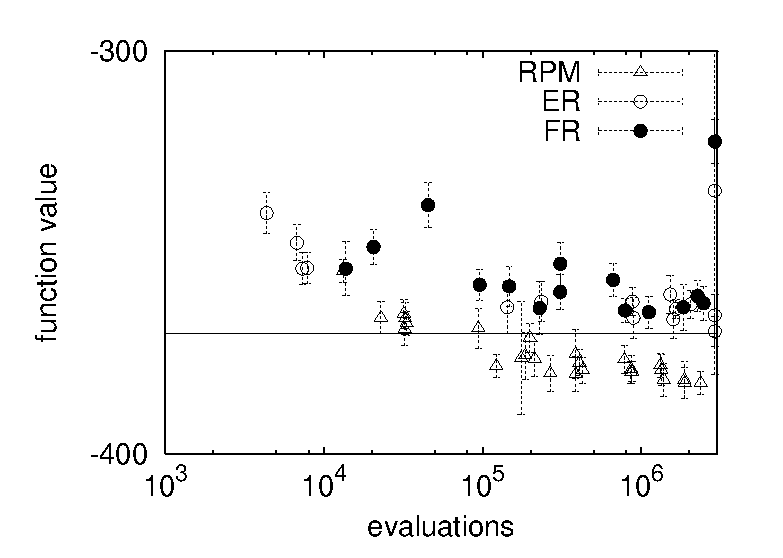
\includegraphics[width=\figlength\linewidth]{data_rpm/idea_vs_rwor_1d.eps}}
\caption{Results for 1D Ising.}
\label{result_1d}
%\end{figure}

\vspace{0.5cm}

%\begin{figure}[tb]
\centerline{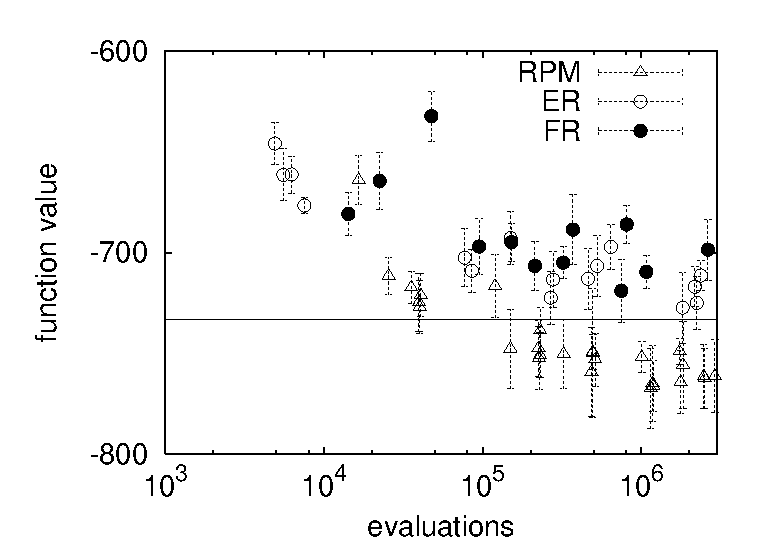
\includegraphics[width=\figlength\linewidth]{data_rpm/idea_vs_rwor_2d.eps}}
\caption{Results for 2D Ising.}
\label{result_2d}
\end{figure}

%\vspace{0.5cm}

\begin{figure}[tb]
\centerline{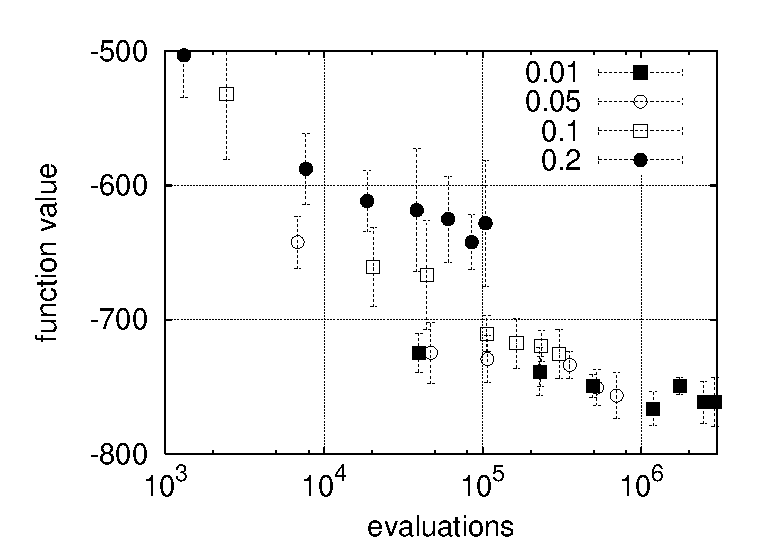
\includegraphics[width=\figlength\linewidth]{data_rpm/rpm_rwor_2d_cutoff.eps}}
\caption{Results of RPM ($N=500$) for 2D Ising.}
\label{result_cutoff}
\end{figure}




\subsection{Comparison with Standard Deviation Schedule}
In this section, ERS with the Boltzmann distribution is compared with SDS,
which is a convergence schedule derived from experimental rule of
genetic algorithms.
SDS is defined by
\begin{equation}
 \beta_{t+1}=\beta_t+\sqrt{\frac{d}{\sigma^2_t}}
\end{equation}
where $\sigma^2_t$ is the variance of the cost function value and
$d$ is a parameter.
If $\beta_t=0$, ERS is equivalent to SDS.
The comparison is also shown in Table \ref{table-erssds}

For each schedule, the parameters are set as
$N=200$ and $M=200$.
For ERS, $c=0.4,~ 0.2,~ 0.1,~ 0.05$.
Note that $\Delta S=\log c$ and the parameter $d$ of SDS corresponds to
$-\Delta S$ if $\beta=0$.
For SDS, $d=-0.001 \times \log c$. 
This is experimentally determined so that
the number of function evaluations taken until the optimization converge
becomes almost the same number.

\begin{table}[tbp]
\renewcommand{\arraystretch}{1.23}
\centering
\caption{Comparison between ERS and SDS}
\large{
\begin{tabular}{|c|c|}
\hline
ERS & $(\beta_{t+1}-\beta_t)^2=\frac{d}{\sigma^2_t} $
\\
\hline
SDS & $\beta_{t+1}^2-\beta_t^2= - \frac{\Delta S}{\sigma_t^2}$ \\
\hline
\end{tabular}
}
\label{table-erssds}
\end{table}


\subsubsection{Result}
Figure \ref{ers_vs_sds_2dising} shows the result.
The vertical axis represents the cost function value of the best
obtained solution.
The horizontal axis represents the number of function evaluations.
The figure shows that
both schedule are almost equivalent in terms of 
the cost function value of the best obtained solution and, however,
ERS consumes slightly smaller number of function evaluations
than SDS.
\begin{figure}
%\vspace{0.1in}
\centerline{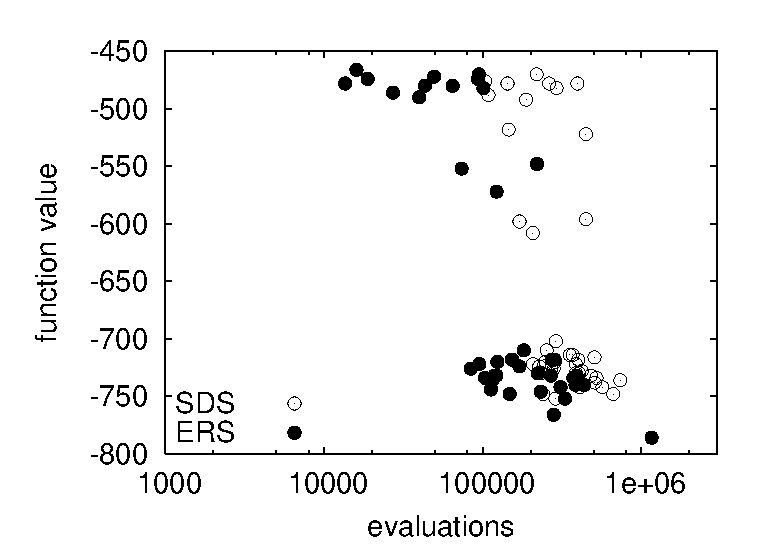
\includegraphics[width=\figlength\linewidth]{data_ers/sds_vs_ers_ising2d.eps}}
\caption{The result of  standard deviation schedule and entropy
 reduction schedule.}
\label{ers_vs_sds_2dising}
\end{figure}


\section{Discussion}
\subsection{Numerical Calculation Error}
In some ideal situations such as the onemax cases,
the entropy of the target distribution can be controlled efficiently.
However, in some cases such as the 1D and 2D Ising cases,
the control of the entropy becomes difficult.
If we have an enough number of samples and enough computational time,
the numerical method for adjusting the threshold or
the inverse temperature can realize the given entropy.
The results show that ERS outperforms SDS.
Hence the numerical method is enough practical 
and this problem of the accuracy of the control may not be important.


\subsection{Linear Time Convergence}
If the entropy is linearly decreased,
the algorithm converge in linear time for an exponential size of the
search space.
Hence, the EAPM with ERS is designed as linear time algorithm.
Unfortunately, there is no guarantee to converge in linear time
because the entropy cannot be controlled precisely in practice.
At least, in our experiments,
the convergence is faster than the theoretical evolution or the almost same.
This property is useful for predicting the convergence time.


\subsection{Application}
Actually, ERS is equivalent to the truncation selection of EDA.
In the EAPM, RPM, and HIS, ERS provides a novel method for controling 
the target distribution.
ERS is a general convergence framework.


\section{Summary}
The entropy reduction schedule (ERS) is based on the following two assumptions:
(1)the target distributions are partially uniform distributions and
(2)the probability models perfectly approximates the target
distributions.
Under these assumptions,
this chapter have revealed the relationship between
entropy and Fisher information.
As a result, we have obtained ERS.

In ERS, the entropy is decreased linearly and
this means linear time convergence for an exponential size of the search
space in theory.
In practice, it is difficult
to exactly realize the target distribution with a given entropy
and the linear time convergence is not guaranteed.
Through experiments, the proposed numerical method seems to work well but not
perfectly and it has been revealed that
ERS outperforms standard deviation schedule.